\section{Errors, Orchestration and Synchronization}

\mnote{Context: categorization and synchronization}
In \autoref{chap:errors}, we have presented and discussed a categorization of errors in transformation networks.
Such errors can occur when different mistakes are made when developing transformation networks, especially missing synchronization of the individual transformations, as discussed in \autoref{chap:synchronization}, but also because an algorithm that applies the transformations is not able to find consistent models because of the orchestration problem, as discussed in \autoref{chap:orchestration}.

\mnote{Empirical evaluation of categorization and synchronization in case study}
We empirically evaluate different aspects of errors, their categorization, and their avoidability as well as resolvability by the discussed approaches in a case study.
In that case study, we utilize a set of independently developed transformations, which were not supposed to be used in a transformation network.
In consequence, executing them in a network leads to several failures.
We analyze these failures and their causes to improve evidence of correctness and completeness of our categorization and to make statements about the relevance of the different failures and causing mistakes by their number of occurrences.
Additionally, we apply our proposed approach for developing synchronizing transformations to resolve the according failures and with that evaluate the correctness and applicability of that approach.

\mnote{Empirical evaluation of practical relevance of orchestration problem}
Since the orchestration problem can always lead to the situation that a transformation application algorithm cannot find consistent models by applying the transformations, we also utilize this case study to investigate how problematic the orchestration problem is actually in practice.
We already know from the halting problem that just because an essential problem in software engineering is undecidable, this must not necessarily be that relevant in practice.


\subsection{Goals and Methodology}

\mnote{Case studies combining existing transformations}
To evaluate both our proposed categorization of errors as well as our presented approach to avoid or find errors, we have conducted two case studies in which we combined existing transformations, of which two were not developed to be used in transformation networks, whereas one was designed to be synchronizing to be used in networks .
In consequence, their combination revealed several errors to evaluate our categorization with and applying our approaches for constructing correct transformation networks, we were able to evaluate the approach for synchronizing transformation construction and the relevance of the orchestration problem as a source of errors.

\mnote{Error identification and correction process}
The general process we followed in those case studies looks as follows:
We combine independently developed transformations and execute existing sets of test cases developed for the individual transformations, which we extended by validations of the further models generated by the additional transformations.
We then validate the failures occurring in the test case execution.
The information about the failures is used to trace back to the causing faults and mistakes, such as missing matchings of elements when multiple instantiations occur.
For each identified failure, we fix the causing fault and re-execute the test cases to validate whether the failure was resolved by fixing the fault.

\mnote{Iterative process because of hidden faults}
The process is applied iteratively until no more failures occur.
Since failures due to one mistake can hide failures of another mistake, it is possible that after fixing all faults that led to the failures in one iteration, still failures occur afterwards.
For example, incompatible consistency relations may not lead to any failure because the scenario fails earlier due to missing element matching. Then, after adding the element matching, the scenario may still fail, but now because of the incompatible consistency relation.
We explain in more detail which transformations we combined in which order in the subsequent section about the case studies.
In the following, we discuss which evaluation goals we achieved with this process and which metrics we employed to answer different questions for achieving that goal.


\subsubsection{Categorization and Orchestration}

\begin{table}
    \centering
    \renewcommand{\arraystretch}{1.4}
    \rowcolors{0}{gray!10}{white}
    \begin{tabular}{p{8em} p{20em}}
        \toprule
        \rowcolor{gray!25}
        \goal{Categorization} & 
            Show that the %relations between mistakes, faults and failures in the categorization for transformation network errors are correct. 
            categorization of mistakes, faults and failures covers all relevant cases and identify relevance of the individual mistake types. \\
        \question[eq:categorization:completeness]{Completeness} & 
            \questiontext{Can all failures be traced back to mistakes according to the categorization?}\\
        \metric & 
            \metrictext{Classified failure ratio: Ratio between classified failures and identified failures} \\
        \question[eq:categorization:correctness]{Correctness} & 
            \questiontext{Are identified failures caused by mistakes they are related to according to the categorization?} \\
        \metric & 
            \metrictext{Resolved failure ratio: Ratio between resolved failures and total failures}\\
        \question[eq:categorization:relevance]{Relevance} & 
            \questiontext{How relevant is each type of mistake, i.e., how likely is it to be made?}\\
        \metric & 
            \metrictext{Mistake type occurrence ratio: Ratio between occurrences of each type of mistake and total occurences of mistakes}\\
        \midrule
        %
    \end{tabular}
    \begin{tabular}{p{8em} p{20em}}
        \rowcolor{gray!25}
        \goal{Orchestration} & 
            Find out how relevant undecidability of the orchestration problem is in practice.\\
        \rowcolors{1}{gray!10}{white}
        \question[eq:orchestration:relevance]{Relevance} & 
            \questiontext{How often does an algorithm for orchestration fail due to the orchestration problem?} \\
        \metric & 
            \metrictext{Fail ratio: Ratio between algorithm failures due to the orchestration problem and all failures} \\
        \bottomrule
    \end{tabular}
    \caption[Goals, questions and metrics for categorization and orchestration]{Goals, questions and metrics for categorization and orchestration evaluation}
    \label{tab:correctness_evaluation:gqm_categorization}
\end{table}

\mnote{Categorization completeness evaluation}
For the evaluation of our error categorization and the relevance of the orchestration problem, we depict the evaluation plan in \autoref{tab:correctness_evaluation:gqm_categorization}.
We evaluate completeness of the categorization in \autoref{eq:categorization:completeness}, i.e., that we did not miss any relevant mistakes in the categorization, by tracing back occurring failures in the case study to causing mistakes. 
This is covered by measuring how many occurring failures could be classified, i.e., traced back to mistakes they were caused by according to the categorization.
The following according metric relates the number of classified to the number of totally identified failures, thus indicating a higher degree of completeness with a higher value with a maximum of $1$:
\begin{align*}
    \mathvariable{classified\ failure\ ratio} = \frac{\mathvariable{\#\ of\ classified\ failures}}{\mathvariable{\#\ of\ total\ failures}}
\end{align*}

\mnote{Categorization correctness evaluation}
Correctness of the categorization, i.e., that failures are actually caused by mistakes they are traced back to in the categorization, is identified by validating whether there are further mistakes that caused the failures in the case study, denoted as \autoref{eq:categorization:correctness}.
This is covered by measuring the number of failures that were resolved by fixing the implementation fault as a consequence of the mistake it was traced back to according to the categorization.
For example, when a failure of multiple instantiations occurs, we search for missing element matches that are the fault caused by the mistake of missing synchronization, to which such a failure can be traced back according to our categorization.
We then measure whether the failure was fixed due to that.
This is reflected by the following metric again indicating a higher degree of correctness with a higher value with a maximum of $1$:
\begin{align*}
    \mathvariable{resolved\ failure\ ratio} = \frac{\mathvariable{\#\ of\ resolved\ failures}}{\mathvariable{\#\ of\ total\ failures}}
\end{align*}

\mnote{Mistake type relevance evaluation}
While we expect correctness and completeness to be given by construction of the categorization, it is unclear without empirical evaluation how relevant the different types of mistakes are, i.e., however often they are likely to be made in actual projects, as defined in \autoref{eq:categorization:relevance}.
This especially influences how important it is to avoid or identify specific types of mistakes.
Therefore, we measure how often each type of mistake leads to a fault in the transformation implementations of the case study and compare it to the total number of mistakes to evaluate their ratio of occurrence.
We reflect this in a metric for each mistake type representing the percentage of all mistakes it made up in the case study:
\begin{align*}
    \mathvariable{mistake\ type\ occurence\ ratio} = \frac{\mathvariable{\#\ of\ mistakes\ of\ type}}{\mathvariable{\#\ of\ total\ mistakes}}
\end{align*}

\mnote{Orchestration problem relevance evaluation}
Finally, directly related to the completeness of our categorization is the relevance of the orchestration problem, discussed in \autoref{chap:orchestration}.
We have seen that a transformation network cannot only fail in delivering consistency models after a change because mistakes led to faults in the single transformations or their combination to a network, but also because the problem of finding a consistent orchestration is, in general, undecidable.
Since our categorization only considers actual mistakes made during network specification and does not reflect the orchestration problem, some failure may not be traceable back to such mistakes, leading to a reduction of completeness as analyzed for \autoref{eq:categorization:completeness}.
We have, however, already discussed in \autoref{chap:orchestration} that it is yet unclear how relevant the orchestration problem is in practice.
Thus, we use the results of our case study to evaluate this relevance as asked in \autoref{eq:orchestration:relevance}.
We measure how often the application algorithm fails to yield consistent models only due to the orchestration problem.
To identify that case, whenever the algorithm fails we validate whether an alternative order of transformation executions would have delivered consistent models.
In fact, not finding such an order would not prove that it does not exist, but we will see that this situation does not occur.
We thus measure the following metric for the ratio of failures due to the orchestration problem:
\begin{align*}
    \mathvariable{fail\ ratio} = \frac{\mathvariable{\#\ of\ failures\ due\ to\ orchestration\ problem}}{\mathvariable{\#\ of\ total\ failures}}
\end{align*}


\subsubsection{Synchronization}

\begin{table}
    \renewcommand{\arraystretch}{1.4}
    \rowcolors{0}{gray!10}{white}
    \begin{tabular}{p{8em} p{20em}}
        \toprule
        \rowcolor{gray!25}
        \goal{Synchronization} & 
            Show that the approach for matching elements avoids failures due to \leveltransformation level mistakes by construction. \\
        \question[eq:synchronization:correctness]{Correctness} & 
            \questiontext{In how many cases does the approach lead to correct synchronizing transformations?} \\
        \metric & 
            \metrictext{Success ratio: Ratio between changes for which no failure due to faults at the \leveltransformation level occurs after applying the approach to all changes for which consistency was not preserved before applying the approach because of faults at \leveltransformation level} \\
        \question[eq:synchronization:completeness]{Completeness} & 
            \questiontext{In how many cases can the approach (not) be applied?} \\
        \metric & 
            \metrictext{Application ratio: Ratio of faults at \leveltransformation level that can be resolved by the approach to all faults at that level}\\
        \bottomrule
    \end{tabular}
    \caption[Goals, questions and metrics for synchronization]{Goals, questions and metrics for synchronization evaluation}
    \label{tab:correctness_evaluation:gqm_synchronization}
\end{table}

\mnote{Evaluation of approach for achieving synchronization}
In addition to the evaluation of our categorization, we also used the case studies to evaluate our approaches for constructing correct transformation networks.
We traced all failures back to the causing mistakes and fixed them according to our proposed approaches.
The analysis of compatibility was evaluated independently in \autoref{chap:correctness_evaluation:compatibility}.
Since it was obvious in all cases in which incompatibilities occurred, we fixed them without running an explicit analysis.
For all failures that could be traced back to missing synchronization, however, we applied our approach presented in \autoref{chap:synchronization:achieving:identification} for making the transformations synchronizing.
This enabled us to evaluate correctness and applicability of our approach to make transformations synchronizing and thus to fix or avoid mistakes at the \leveltransformation level.

\mnote{Synchronization correctness evaluation}
We first measures whether the proposed approach for matching existing elements is correct, i.e., whether it leads to synchronizing transformations. This is covered by \autoref{eq:synchronization:correctness}.
To measure this, we counted the test cases in which failures occurred because of faults that were made at the \leveltransformation level leading to missing synchronization and that we could fix by adding missing element matching.
We applied our approach, i.e.k we added added the missing element matchings, and counted in how many cases this resolved all failures due to faults at the \leveltransformation level.
This is covered by a metric that represents the success rate of the approach:
\begin{align*}
    \mathvariable{success\ ratio} = \frac{\mathvariable{\#\ of\ tests\ with\ resolved\ failures\ after\ approach\ application}}{\mathvariable{\#\ of\ tests\ due\ to\ which\ approach\ was\ applied}}
\end{align*}
In fact, we only count the test cases after applying the approach which failed before due to faults at the \leveltransformation level, because we are only interested in test cases that failed before and otherwise the metrics could become larger than $1$.

\mnote{Synchronization completeness evaluation}
In the correctness evaluation, we only counted the tests in which we were able to apply our approach.
This was on purpose because it may be possible that the approach cannot be applied in all cases.
First, this can be due to the fact that there is no unique information to match existing elements (see \autoref{chap:synchronization:achieving:identification}).
Second, we may have missed further reasons than missing matching of existing elements preventing the transformations from being synchronizing.
Both cases would restrict the completeness of our approach as considered by \autoref{eq:synchronization:completeness}, because it would not be possible to resolve or avoid all possible failures due to missing synchronizing by adding matchings for existing elements.
To measure this, we counted the number of faults at the \leveltransformation level that we were not able to resolve to the total number of faults:
\begin{align*}
    \mathvariable{application\ ratio} = \frac{\mathvariable{\#\ of\ resolved\ faults\ at\ \leveltransformation\ level}}{\mathvariable{\#\ of\ total\ faults\ at\ \leveltransformation\ level}}
\end{align*}
Although we applied the approach for achieving synchronizing transformations after identifying that transformations are non-synchronizing rather than applying the approach to specify transformations that are synchronizing by construction, the results regarding correctness and completeness still apply if the approach is applied during transformation construction.
%Additionally, we have used one transformation that was developed to be used in a transformation network by applying the matching of existing elements already 


% We have systematically constructed the categorization in \autoref{chap:errors} from the potentials for mistakes that are induced by the different specification levels. % we identified (\autoref{sec:process:levels}).
% To further improve evidence regarding completeness and correctness of %the identified mistakes, resulting failures and their dependencies, we validate that 
% our categorization, we validate it in a case study as our contribution~\ref{contrib:evaluation}.
% The goal is 
%  to show completeness of the identified mistakes and failures, and
%  to investigate correctness of the dependencies between them. % mistakes and resulting failures. %,
 %and to show appropriateness of the strategies for avoiding mistakes presented in \autoref{sec:avoiding}.

% Evaluation goals:
% \begin{itemize}
%     \item Completeness of identified mistakes/failures
%     \item Correctness of dependencies between failure types and mistakes
%     \item Appropriateness of matching strategy for avoiding operationalization issues
% \end{itemize}

% \subsubsection*{Process}
% We executed the test cases on a transformation network, which we created as a combination of the existing transformations.
% They were executed until no further changes occurred.
% We then classified the occurring failures according to \autoref{chap:errors:failures}.
% Based on our categorization in \autoref{chap:errors:categorization}, we traced back the failures to mistakes and fixed them according to the strategies discussed in \autoref{chap:prevention}.
% Failures can be hidden by others: 
% For example, an incompatible constraint may produce no failure because the scenarios fail earlier due to missing element matching or vice versa.
% For this reason, we re-executed the process until no further failures occurred.
% Finally, we applied the transformations to the more complex Media Store construction case to validate that all mistakes were fixed.

% \subsubsection*{Measurements}
% We measured the number of failures in each of the iterations.
% We relate the number of failures that we were able to categorize to the total number of recognized failures ($\mathit{identifiedFailureRatio} = \frac{\mathit{\#\ of\ categorized\ failures}}{\mathit{\#\ of\ total\ failures}}$) to show completeness of the identified failure types.
% This metric is rather weak, because it does not identify whether a failure is categorized correctly.
% We therefore relate the total number of resolved failures, which are those that do not occur in the subsequent iteration anymore, to the number of detected failures ($\mathit{resolvedFailureRatio} = \frac{\mathit{\#\ of\ resolved\ failures}}{\mathit{\#\ of\ total\ failures}}$).
% If a failure disappears after fixing the causing mistakes, the classification of the failure and also the relation to the causing mistake was correct. %, which is why this metric gives an indicator for the completeness of the identified failure types.
% Therefore, this metric gives an indicator for both completeness of the identified failure types and the relation of mistakes to failures.

%To measure correctness of the dependencies between mistakes and failures, we relate the resolved mistakes to the detected failures ($\frac{\text{# of resolved mistakes}}{\text{# of detected failures}}$.
%If the number of resolved mistakes is lower than the number of failures, actually failures remain after fixing an mistake, which indicated that some relation between mistake and failure type was wrong.



\subsection{Prototypical Implementation}
% Context of the implementation, actual implementations

\mnote{\vitruv framework for implementation}
For the conduction of the case studies presented in the subsequent section, we have used a prototypical implementation in the \vitruv framework (see \autoref{chap:foundations:multiview:vitruv})~\cite{klare2020Vitruv-JSS}.
It support the view-based development of consistent systems by managing a consistent representation of all information about a software systems, from which views can be derived to be modified by the user.
Internally, the system is represented as a set of models of existing or newly defined languages, which are kept consistent by means of bidirectional model transformations.
The transformations operate in an incremental and delta-based way. 
It is incremental, because it updates the existing models rather than creating new ones upon changes.
It operates delta-based, as is does not receive the modified state of a model, but a delta between the old and the new state.
This conforms to what we introduced as a change in our formalism (see \autoref{def:change}).
To achieve this, the framework records atomic changes to the models, i.e., element creations and deletion, as well as attribute and references changes, as discussed in \autoref{chap:synchronization:achieving:changes} and depicted in \autoref{fig:synchronization:change_feature_model}, and passes them to the transformations.
Currently, it lacks support for the combination of multiple transformation to a network for keeping multiple models consistent, which is why we implemented our approaches in a case study with that framework.

\mnote{\reactionslanguage for unidirectional consistency preservation rules}
The \vitruv framework provides, among others, the \reactionslanguage~\cite{klare2016b,langhammer2017a} for defining unidirectional consistency preservation rules according to \autoref{def:unidirectionalconsistencypreservationrule}.
Defining such unidirectional rules for both directions between two metamodels yields a bidirectional transformation according to \autoref{def:bidirectionaltransformation}.
These transformations only have an explicit representation of the consistency preservation rules, whereas the consistency relations are only implicitly defined as the fixed points of the application of the consistency preservation rules.
We use the \reactionslanguage for implementing consistency preservation in our case studies.

\mnote{\reactionslanguage uses correspondence model}
The \reactionslanguage uses a so called \emph{correspondence model} to identify corresponding elements according to the implicitly defined consistency relations and thus implements a witness structure according to \autoref{def:consistency}.
It enables to trace when elements were changed to update the corresponding element rather than always deleting and adding a corresponding element.
We have discussed in TODO that this still conforms to our formalism, although we did explicitly omitted any kind of trace model there.
\todo{Add reference to discussion about trace model in correctness chapter}

\lstinputlisting[%
float,%
language=reactions,
caption={\reaction creating a \gls{UML} class among creation of a \gls{PCM} component. Adapted from \cite{klare2020Vitruv-JSS}.},
label={lst:correctness_evaluation:errors:reaction_example},
escapechar=~
]{listings/correctness/evaluation/reaction_example.tex}

\mnote{Example for \reactions}
A transformation rule defined in that language is called a \emph{\reaction}.
To give an impression of how such rules look like, an example that transforms a \gls{PCM} component into a class with appropriate naming in \gls{UML} among its creation is depicted in \autoref{lst:correctness_evaluation:errors:reaction_example}.
A \reaction specifies after which type of change it should be executed, which, in this case, is the insertion of a component into a repository.
It may then call one or more reusable \emph{routines} that are supposed to restore consistency according to a consistency relation.
Such a routine consists of a \emph{match} block, which checks whether a consistency relation applied and retrieves all elements involved into that relation, and an \emph{action} block, which restores consistency after the change.
In this case, the routine checks that no corresponding class already exists to avoid multiple instantiation and afterwards retrieves an appropriate package in the \gls{UML} model to place the class in.
It then creates a class, assigns it an appropriate name and adds a correspondence between the elements.
For the complete explanation of that example, we refer to \cite{klare2020Vitruv-JSS}.

\mnote{Simple orchestration strategy}
In \autoref{chap:orchestration}, we have discussed different options for the orchestration of transformations in an application algorithm.
In the \vitruv framework, we have implemented a simple depth first execution of transformation without an artificial execution bound.
This means, for a given change all transformation involving that changed model are executed consecutively.
After the execution of each transformation, this approach is recursively applied to the model changed by that transformation, which implements the depth-first execution.
If the model is not changes, i.e., if the models are already consistent, the recursion aborts.
This finally finishes the algorithm.
This results in an algorithm comparable to the provenance algorithm proposed in \autoref{chap:orchestration:algorithm}. as it implements a similar recursion strategy
In contrast, the implemented strategy, however, does not only consider already executed transformations in the recursion and does not define an execution bound.
In fact, that implementation may not terminate.

\mnote{Implicit consistency relations in \reactionslanguage}
Since the transformations defined in the \reactionslanguage only contain implicit consistency relations by the fixed points of their consistency preservation rules, checking consistency for the recursion to abort is conducted by checking whether the transformation performed any changes.
If this is not the case, the models are considered correct by construction.
We have already discussed this as an option for the realization of a \function{CheckConsistency} function within an application algorithm in \autoref{chap:orchestration:decidability:algorithm}.
The implementation of the framework with the \reactionslanguage is available in a GitHub repository~\cite{vitruvFrameworkGithub}.

%\todo{Note that the Vitruv implementation has no CheckConsistency method but uses hippocratic transformations and aborts if no further changes occur by executing the transformations. Thus consistency relations are implicitly encoded in the consistency preservation rules by being their fixed points.}

%Wir betrachten Transformation in Reactions.
%Synchronisation durch mehrfache Ausführung der Transformationen in beide Richtungen.

%Depth-first propagation von Änderungen.

%Orchestrierung: FIFO für Transformationen, an denen Modelle geändert wurden. Kein Abbruchkriterium, d.h. es kann zu Nicht-Terminierung kommen. Aber: nach Korrigieren der Fehler keine Nicht-Terminierung mehr (obwohl das nicht so sein muss, siehe Orch-Kapitel). 

\begin{copiedFrom}{ICMT}



\subsection{Case Studies}

\mnote{Transformations for \gls{PCM}, \gls{UML} and Java}
We have performed two case studies based on one set of metamodels and transformations between them defined in the \reactionslanguage.
The case study employs the metamodels \gls{PCM} for component-based software architecture descriptions, \gls{UML} for object-oriented software design, and Java for source code development.
Transformations are defined between each pair of these metamodels, based on consistency relations that we discuss in more detail in the following.
We haven chosen these metamodels and transformations for our case studies, because except for one transformation they were explicitly developed independently without the goal of using them within a transformation network, yielding the possibility to evaluate our categorization and resolution approaches.
The transformations even assumed that they are only executed in one direction after a user change.
It is difficult to find further comparable examples, because we require transformations whose induced graph contains cycles as otherwise most of the discussed problems do not occur at all.
If such transformations exist, however, they were usually defined in a way that they properly work together, as otherwise they would not be usable at all.

\mnote{Two sets of underlying consistency relations}
The used transformations rely on two sets of consistency relations.
First, the relations between \gls{PCM} and object-oriented design in both \gls{UML} and Java were defined by and explained in detail by \textcite{langhammer2015a, langhammer2017a}.
He, in particular, proposed different options for relations between \gls{PCM} and Java, which can be generalized to object-oriented design.
We selected the mapping of architectural components to classes as the one which was most intensively studies and whose implementation is most mature.
Second, the relations between \gls{UML} and Java reflect the usually implicitly known mapping between the two languages, as both describe the object-oriented structure of a software system in a similar way.

\begin{table}
	\centering 
    \small
    \renewcommand{\arraystretch}{1.4}
    \rowcolors{2}{gray!10}{}
	\begin{tabular}{p{3.2cm} p{6.6cm}}
		\toprule
        \textbf{\gls{PCM} Element}  & \textbf{Object-oriented Design Element} \\
        \midrule
		Repository              & Three packages: main, contracts, data types\\
		BasicComponent 		    & Package within the main package and a public component realization class within the package \\
		OperationInterface		& Interface in the contracts package \\
		Signature \& parameters & Method \& parameters \\
		CompositeDatatype       & Class with getter and setter (or appropriate read-only property) for inner types\\
		CollectionDatatypes     & Class that inherits from a collection type (e.g. \texttt{ArrayList} in Java) \\
		RequiredRole		    & Field typed with required interface in the component realization class and constructor parameter for the field in the component realization class\\
		ProvidedRole		    & Component realization class of providing component implements the provided interface\\
		\bottomrule
	\end{tabular}
	\caption[Consistency relations between PCM and UML/Java]{Consistency relations between elements of the \gls{PCM} repository metamodel and object-oriented design elements (\gls{UML}/Java), adapted from \cite[Table 4.1]{langhammer2017a}.}
	\label{tab:correctness_evaluation:errors:pcm_oo_rules}
\end{table}

\mnote{Relations between \gls{PCM} and object-oriented design}
\autoref{tab:correctness_evaluation:errors:pcm_oo_rules} shows the relevant consistency relations between \gls{PCM} models and object-oriented design, which can be reflected in both \gls{UML} and Java.
A \gls{PCM} repository model consists of data types, interfaces and components, which are all contained in one repository.
The repository is represented as a package structure in object-oriented design.
Components are represented as a package containing a so called \emph{component realization class}.
Interfaces with their signatures and parameters are mapped to corresponding object-oriented elements as they are.
Composite data types are represented as a class containing the composed types and collection data types are represented as subclasses of any collection type.
Finally, provided and required roles define that a component provides or requires an interface.
Provided roles are realized by an implementation of the provided interfaces in the component realization class.
Requires roles, on the contrary, are represented as a field in the component realization class, which must be set via constructor parameter.

\mnote{Transformations between \gls{PCM} and \gls{UML}, as well as \gls{PCM} and Java}
The preservation of consistency between \gls{PCM} and Java according to these relations using the \reactionslanguage was implemented in the Master's thesis of this thesis' author~\cite{klare2016b} in the context of the dissertation of \textcite{langhammer2017a}.
At that point in time, the transformation was only defined to be executed once in one direction and, in particular, not to be used in a transformation network.
In addition, \citeauthor{syma2018ma} defined the bidirectional transformation between \gls{PCM} and \gls{UML} in his Master's thesis~\cite{syma2018a}.
He also proposed a formal specification of those relations and their preservation~\cite[Section 5]{syma2018ma}.
This transformation was defined to be used in a transformation network and therefore implement the matching of existing elements according to \autoref{chap:synchronization:achieving:identification} to achieve synchronization of the transformation.

\mnote{Exclusion of behavioral consistency between \gls{PCM} and Java}
Actually, \gls{PCM} models can also contain \emph{service effect specifications}, which are an abstract specification of the behavior of a service provided by a component.
Consistency between these behavior specifications in \gls{PCM} and their implementation in Java code was researched in detail by \textcite{langhammer2017a} and is one of the reasons why in this scenario consistency between \gls{PCM} and Java cannot only be expressed across \gls{UML}.
We do, however, not consider that consistency relation in this case study, because we focus on structural consistency relations, as motivated in \autoref{chap:networks:notions:types}.
Since these behavioral descriptions share an isolated relation between \gls{PCM} and Java, it is not relevant for our considerations on transformation networks anyway.

\begin{table}
	\centering 
    \small
    \renewcommand{\arraystretch}{1.4}
    \rowcolors{2}{gray!10}{}
	\begin{tabular}{p{3cm} p{6.8cm}}
		\toprule
        \textbf{\gls{UML} Element}  & \textbf{Java Code Element} \\
        \midrule
        Package                         & Package\\
		Class                           & Class\\
		Enum		                    & Enum \\
		Interface		   	            & Interface \\
        Method                          & Method \\
        Parameter $[$0-1 .. 1$]$        & Parameter of same type \\
        Parameter $[$0-* .. 2-*$]$      & Parameter of collection type with type parameter \\
        Field $[$0-1 .. 1$]$            & Field of same type\\
        Field $[$0-* .. 2-*$]$          & Field of collection type with type parameter\\
        Association $[$0-1 .. 1$]$      & Field of same type\\
        Association $[$0-* .. 2-*$]$    & Field of collection type with type parameter\\
		\bottomrule
	\end{tabular}
	\caption[Consistency relation between UML and Java]{Consistency relations between \gls{UML} class models and Java code.}
	\label{tab:correctness_evaluation:errors:uml_java_rules}
\end{table}

\mnote{Relations between \gls{UML} and Java}
\autoref{tab:correctness_evaluation:errors:pcm_oo_rules} shows the relevant consistency relations between \gls{UML} models and Java models.
They reflect the intuitive notion of the relation between \gls{UML} and Java of mostly one-to-one mappings, since we do only consider Java elements that are present in the abstraction provided by the \gls{UML}, i.e., we especially do not consider method bodies.
The only special cases are fields having a type of another class in Java classes, which can also be expressed as associations in \gls{UML}, as well as parameters, fields and associations, which can have multiplicities in \gls{UML} that have to be expressed as collection types with an appropriate type parameter in Java if the upper bound is higher than 1.

\mnote{Transformations between \gls{UML} and Java}
The preservation of consistency between \gls{UML} and Java according to these relations was implemented using the \reactionslanguage within a Bachelor's thesis supervised by the author of this thesis.
Like for the transformation between \gls{PCM} and Java, this one was implemented to be used in one direction only and thus, especially, not to be used in a transformation network.

\mnote{Implementation of transformations with test cases}
The implementations of all transformations are available in a corresponding GitHub repository of the \vitruv project~\cite{vitruvCBSEGithub}.
Each of them also contains a sophisticated set of test cases, which were supposed to test each transformation only executed in one direction after changes to one model.
We reused and extended these test cases for our case study.
This setup of independently developed transformations and test cases ensures that there is only low risk of the transformations and test cases to be initially aligned with each other, which could result in a bias of the results.

\begin{table}
    \centering
    \small
    \renewcommand{\arraystretch}{1.4}
    \rowcolors{2}{}{gray!10}
    \begin{tabular}{L{7em}C{4em}C{4em}C{4em}}
        \toprule
        \textbf{$\downarrow$ From} / \textbf{To $\rightarrow$}& \gls{PCM} & \gls{UML} & Java \\
        \midrule
        \gls{PCM} & -   & 57    & 40 \\
        \gls{UML} & 68  & -     & 63 \\
        Java      & 16  & 49    &   \\
        \bottomrule
    \end{tabular}
    \caption[Complexity of case study transformations]{Complexity of the case study transformations in terms of the number of \reactions in each consistency preservation rule, i.e., the number of change types it is able to react to.}
    \label{tab:correctness_evaluation:errors:study_complexity}
\end{table}

\mnote{Complexity of case study transformations}
To give an impression of the complexity of the transformations, we depict the number of \reactions in each of the six unidirectional consistency preservation rules in \autoref{tab:correctness_evaluation:errors:study_complexity}.
This conforms to the number of change types each of these consistency preservation rules is able to react to.
The lower number of \reactions between Java and \gls{PCM} is mainly due to the fact that several elements of the \gls{PCM} are mapped to the same elements in Java.
For example, components and all kinds of data types are mapped to classes in Java, such that the \reactions in Java must react to less change types and instead make more distinctions within the routines to separate the affected consistency relations.


\todo{Go on here}

Zwei Case Studies (Torsten/Timur)
\gls{PCM}

\begin{table}
    \centering
    \small
    \renewcommand{\arraystretch}{1.2}
    \begin{tabular}{L{13em}C{8em}}
        \toprule
        \textbf{Consistency Relation} & \textbf{\# of Test Cases} \\
        \midrule
    \end{tabular}
    \rowcolors{1}{}{gray!10}
    \begin{tabular}{L{13em}C{8em}}
        \textit{\gls{PCM} $\leftrightarrow$ \gls{UML} Core}\\\addlinespace[0.3em]
        Repository              & $4$ \\
        Interface               & $2$ \\
        System                  & $2$ \\
        Composite Data Type     & $4$ \\
        Repository Component    & $2$ \\
        Assembly Context        & $2$ \\\addlinespace[0.3em]
        \rowcolor{gray!25}
        \textbf{Total}          & $\mathbf{16}$ \\
        \midrule
    \end{tabular}
    \rowcolors{1}{}{gray!10}
    \begin{tabular}{L{13em}C{8em}}
        \textit{\gls{PCM} $\leftrightarrow$ \gls{UML} Additional}\\\addlinespace[0.3em]
        Signature       & $6$ \\
        Parameter       & $6$ \\
        Attribute       & $6$ \\
        Required Role   & $3$ \\
        Provided Role   & $2$ \\\addlinespace[0.3em]
        \rowcolor{gray!25}
        \textbf{Total}  & $\mathbf{23}$ \\
        \midrule
    \end{tabular}
    \rowcolors{1}{}{gray!10}
    \begin{tabular}{L{13em}C{8em}}
        \textit{\gls{UML} $\leftrightarrow$ Java} \\\addlinespace[0.3em]
        Package                     & $6$ \\
        Class                       & $23$ \\
        Enum                        & $14$ \\
        Interface                   & $10$ \\
        Class Method + Parameter    & $29$ \\
        Interface Method            & $9$ \\
        Class                       & $19$ \\\addlinespace[0.3em]
        \rowcolor{gray!25}
        \textbf{Total}              & $\mathbf{110}$ \\
        \bottomrule
    \end{tabular}
    \caption[Number of test cases for case studies]{Number of test cases for the different consistency relations in the case studies.} % Partly taken from \cite[Table 4.1]{saglam2020ma}.} 
    \label{tab:correctness_evaluation:errors:test_cases}
\end{table}

Ausgangspunkt: Tests der uni/bidirektionalen Transformationen

Call it single transformation study
Torsten: Betrachtung der isolierten Erstellung von bidirektionalen aus unidirektionalen Transformationen
Trotz Linearität, also keine zusammenlaufenden Propagationspfade, Probleme auf Transformationsebene, weil jede unidirektionale Transformation schon nicht davon ausgegangen ist, dass es mit einer anderen unidirektionalen Zusammenarbeiten muss.
Das ist äquivalent dazu, wenn mehrere Transformationen zusammenlaufen, da dort die Transformation nicht davon ausgeht, dass eine andere Elemente erzeugt hat, und hier die Transformation nicht davon ausgeht, dass die Rückrichtung die Elemente erzeugt hat, sondern denkt, dass die Informationen immer vom Nutzer kommen.
Hier fehlte also nicht nur die Prüfung über implicit unique information, wie in \autoref{chap:synchronization:achieving:identification} eingeführt, sondern bereits die Prüfung über explicit unique information (Korrespondenzen) bzgl. der Existenz von Elementen.

PCM<>UML direkt mit Patterns entwickelt, UML<>Java nicht, daher hohe Anzahl Fehler in letzterem -> genauer gesagt PCM/UML direkt bidirektional entwickelt, UML/Java nicht, daher dort Unidirektionalitätsfehler (s.u.)
Änderungen an allen Domänen ausgeführt, insbesondere Media Store-Instanzen in jeder Domäne eingespielt.

PCM-UML: 39 tests
UML-Java: 110 tests
+ 5 Tests for MediaStore creation as PCM and UML model
In total, we have used 187 (sic!) test cases that perform different kinds of relevant fine-grained changes in instances of all metamodels, such as insertions, modifications and deletions of all types of elements that have to be kept consistent.
Additionally, we have simulated the construction of the Media Store system~\cite{strittmatter2016a}, which is a sophisticated case study system for the \ac{PCM}.
This system is available as a \ac{PCM} model as well as Java code.

Unterschiedliche Anzahl durch unterschiedliche Granularität der Testfälle


Call it network study
Timur: Kopplung der bidirektionalen Transformationen zu Netzwerken
All tests triggered by changes to PCM.
Started with PCM<>UML tests, then consecutively added transformations, first UML/Java, each direction on its own, then PCM/Java each direction on its own.


\begin{figure}
    \centering
    \newcommand{\arrowshift}{0.3em}
\begin{tikzpicture}[
    mm/.style={draw, minimum height=2em, minimum width=5em}
]
    \node[mm] (pcm) {PCM};
    \node[mm, right=16em of pcm.center, anchor=center] (uml) {UML};
    \node[mm, below right=4.5em and 8em of pcm.center, anchor=center] (java) {Java};
    \draw[-latex] ([yshift=\arrowshift]pcm.east) -- ([yshift=\arrowshift]uml.west);
    \draw[-latex] ([yshift=-\arrowshift]uml.west) -- ([yshift=-\arrowshift]pcm.east);
    \draw[-latex] ([xshift=1.4*\arrowshift]uml.south) -- node[below right] {1.} ([yshift=-1.4*\arrowshift]java.north east);
    \draw[-latex] ([xshift=-1.4*\arrowshift]java.north east) -- node[above left] {2.} ([xshift=-2*\arrowshift]uml.south);
    \draw[-latex] ([xshift=-1.4*\arrowshift]pcm.south) -- node[below left] {3.} ([yshift=-1.4*\arrowshift]java.north west);
    \draw[-latex] ([xshift=1.4*\arrowshift]java.north west) -- node[above right] {4.} ([xshift=2*\arrowshift]pcm.south);
\end{tikzpicture}
    \caption[Phases of second case study]{Phases of the network study by depicting the transformations that are incrementally added in each of the phases.}
    \label{fig:correctness_evaluation:errors:study_phases}
\end{figure}


% The evaluation is based on a case study developed for the Ecore-based \textsc{Vitruvius} framework~\cite{kramer2013b} for consistent system development, which is available on GitHub~\cite{vitruvFrameworkGithub}.
% \textsc{Vitruvius} uses incremental, delta-based consistency preservation. 
% It records atomic changes in models and executes consistency preservation specifications, according to \autoref{def:consistency_preservation_specification}, to inductively preserve consistency.
% Those specifications are written in the Reactions language~\cite{klare2016b}, which is a language for unidirectional transformations at the operationalization level.

% The case study is based on consistency between UML class models, instances of the \ac{PCM}, which is an architecture description language for performance prediction~\cite{reussner2016b}, and Java code.
% For these metamodels, different persons have independently developed transformations~\cite{kramer2017a}, especially without knowing about the other transformations with which they shall be combined.
% This made the specifications prone to mistakes at the modularization and operationalization level.
% The specifications are available on GitHub~\cite{vitruvCBSEGithub}.
% For the evaluation, we employ the pairs of unidirectional specifications between \ac{PCM} and UML, as well as between UML and Java.
% Although this induces only two bidirectional specifications, we have four transformations since both directions of the transformations have been specified independently.
% They have to interoperate correctly, may also contradict, and need to perform element matching.
% % In consequence, this is not a drawback or threat in contrast to a case study of at least three independently developed \acp{BX} that are prone to interoperability issues (apart from the fact that it is hard to find such a case study).
% Thus, our scenario is prone to the same mistakes as a scenario with three or more \acp{BX}.

% The transformations realize rather trivial constraints between UML and Java.
% Most elements are mapped one-to-one, whereas multi-valued parameters and associations are mapped to collection types in Java.
% The relations between \ac{PCM} and UML were proposed by \textcite{langhammer2015a}.
% Interfaces are equally represented, \ac{PCM} components and data types are mapped to classes in UML.
% %Interfaces and data types are mapped to their counterparts in the different metamodels.
% \ac{PCM} components contain \acp{SEFF}, which are an abstraction of their behavior specification used for performance prediction. 
% Those \acp{SEFF} are mapped to methods in UML and Java.
% In total, the transformations between \ac{PCM} and UML react to 57 change types in \ac{PCM} and 65 change types in UML, and the transformations between UML and Java react to 66 change types in UML and to 48 change types in Java to restore consistency in the other model.
%consist of reactions to 57 change events in \ac{PCM} that restore consistency to UML, reactions to 67 change types in UML that restore consistency in \ac{PCM}, reactions to 55 change types in UML that restore consistency in Java, and reactions to 48 change types in Java that restore consistency in UML.

% In total, we have used 187 test cases that perform different kinds of relevant fine-grained changes in instances of all metamodels, such as insertions, modifications and deletions of all types of elements that have to be kept consistent.
% Additionally, we have simulated the construction of the Media Store system~\cite{strittmatter2016a}, which is a sophisticated case study system for the \ac{PCM}.
% This system is available as a \ac{PCM} model as well as Java code.

% \begin{itemize}
%     \item Used environment: Implementation in the Ecore-based Vitruvius framework \cite{kramer2013b}~\footnote{\url{http://vitruv.tools}} for consistent system development
%     \begin{itemize}
%         \item incremental, inductive, delta-based consistency preservation: recording atomic changes, executing consistency preservation specifications for them, as defined in \autoref{def:consistency_preservation_specification}
%         \item specifications in the Reactions language (definition on operationalization level)
%     \end{itemize}
%     %\item Application strategy: batch, Depth-first, finally irrelevant, as same mistakes can occur with any strategy
%     \item Metamodels and consistency preservation specifications:
%     \begin{itemize}
%         \item UML, PCM and Java
%         \item Existing specifications: UML $\leftrightarrow$ Java, PCM $\leftrightarrow$ UML, PCM $\leftrightarrow$ Java
%         \item Independently developed, without knowledge about combined execution $\rightarrow$ black-box development
%         \item So during combined execution mistakes on modularization and operationalization level possible
%     \end{itemize}
%     \item Evolution scenarios:
%     \begin{itemize}
%         \item Test suite of \FIXME tests each making different kinds of small changes
%         \item Simulation of construction of example system: Media Store \cite{strittmatter2016a, reussner2016b}, a case study for PCM with existing specifications in PCM and Java
%     \end{itemize}
% \end{itemize}



\subsection{Results and Interpretation}

Complete overview in thesis of Timur.
Make matrix of mistake types and stages with associated numbers of faults and failures.



Torsten: 159 failures
154 failures (multiple instantiation) -> 25 missing matchings
3 failures (non termination with divergence) -> 1 incompatible constraint (fully qualified vs. simple name)
2 failures (non termination with alternation) -> 1 option selection (visibilities between UML and Java)
Incompatibilities because of two unidirectional consistency relations that are conflicting.


Timur: 118 failure
37 failures (inconsistent termination) -> 12 incorrect transformations
57 failures (multiple instantiation) -> 13 missing matchings
24 failures (multiple instantiation) -> 4 incompatible constraints (contradicting name constraints, therefore duplications)

\todo{Tabelle mit Gegenüberstellung von Failures und Faults machen. Daraus auch kurz analysieren, welche Faults wie viele Failures produzieren.}
Incorrect transformation are out of scope. Were not counted in first case study.
There are more failures because of missing matching than test cases exist, because some test cases failed after fixing one missing match again because of another missing match.
The exact number of each missing match can be found in the MA of Timur.

\todo{Analyisieren zu wie vielen Failures ein Mistake führt}

\subsubsection{Categorization}

Completeness: All failures could be traced back to mistakes of the categorization, most importantly missing matchings and incompatible constraints.
We do not consider the incorrect transformations, because transformations were assumed to be correct, thus these occurrences reflect a different problem than we want to consider.
In total, we found 277 failures. The number of failures is higher in the first case study because more test cases were executed there.
Finally, it does not matter because the $\mathvariable{classified failure ratio} = 1$.
Indicating completeness of the categorization as considered in \autoref{eq:categorization:completeness}.

Additionally, all failures were fixed after fixing the causing faults that were implemented because of the mistakes we identified.
We fixed the missing matchings, the incompatible constraints and the selection of options and found that all tests pass afterwards.
Thus we also have $\mathvariable{resolved failure ratio} = 1$.
Indicating correctness of the categorization as considered in \autoref{eq:categorization:correctness}.

Very interesting are the results regarding relevance of the individual mistakes types.

\begin{figure}
    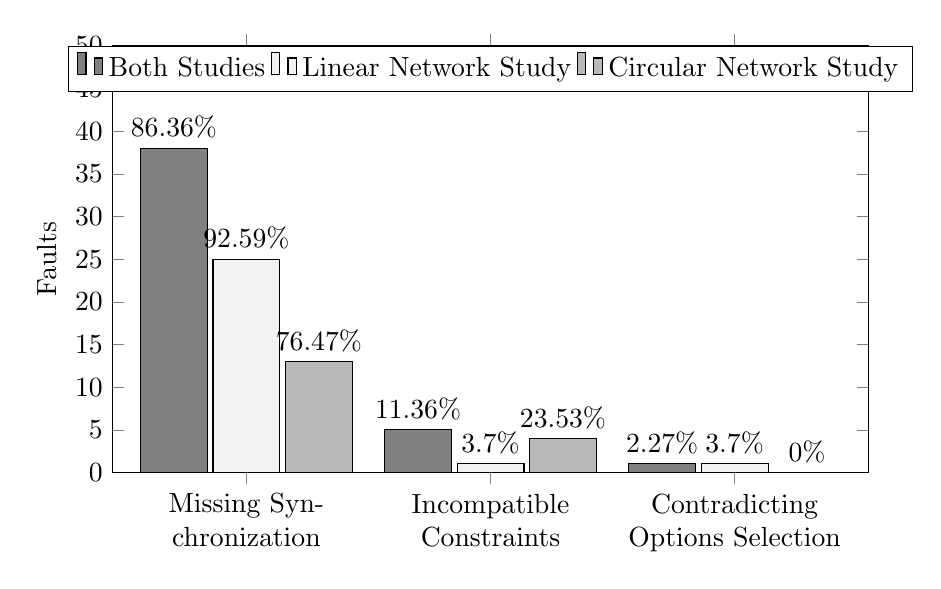
\begin{tikzpicture}
    \begin{axis}[
        ybar,
        bar width=0.85cm,
        x=3.1cm,
        height=7cm,
        legend style={at={(0.5,1)},anchor=north,legend columns=-1},
        ylabel={Faults},
        symbolic x coords={Missing Synchronization, Incompatible Constraints, Contradicting Options Selection},
        xticklabel style={text width=2.8cm, align=center},
        xtick=data,
        ytick distance=5,
        ymin=0,
        ymax=50,
        enlarge x limits={abs=1.7cm},
        nodes near coords align={vertical},
    ]
    \addplot[fill=gray,
        point meta={y*100/44}, % 44 Mistakes in total, calculate percentage
        nodes near coords={\pgfmathprintnumber\pgfplotspointmeta\%},
        ] table[x=Mistake Type, y=occurrences, col sep=comma] {
            Mistake Type,                       occurrences
            Missing Synchronization,            38
            Incompatible Constraints,           5
            Contradicting Options Selection,    1
        };
    \addplot[fill=gray!10,
        point meta={y*100/27}, % 27 Mistakes in total, calculate percentage
        nodes near coords={\pgfmathprintnumber\pgfplotspointmeta\%},
        ] table[x=Mistake Type, y=occurrences, col sep=comma] {
            Mistake Type,                       occurrences
            Missing Synchronization,            25
            Incompatible Constraints,           1
            Contradicting Options Selection,    1
        };
    \addplot[fill=gray!55,
        point meta={y*100/17}, % 17 Mistakes in total, calculate percentage
        nodes near coords={\pgfmathprintnumber\pgfplotspointmeta\%},
        ] table[x=Mistake Type, y=occurrences, col sep=comma] {
            Mistake Type,                       occurrences
            Missing Synchronization,            13
            Incompatible Constraints,           4
            Contradicting Options Selection,    0
        };
        \legend{Both Studies, Linear Network Study, Circular Network Study}
    \end{axis}
\end{tikzpicture}
    \caption[Number of occurrences of mistake types]{Absolute and relative number of occurrences of different mistake types in both case studies.}
    \label{fig:correctness_evaluation:errors:mistake_type_numbers}
\end{figure}

Relevance: Most relevant is synchronization, then compatibility, option selection occurred seldom and not other problems in case study
Although no option selection mistake in different, larger study, there was one in the first, only considering bidirectional transformations. Thus, we can expect this to be relevant for networks as well, even if it did not occur in the case study.
In answer to \autoref{eq:categorization:relevance}, we can see that missing synchronization is the most relevant mistake type, followed by incompatibilities.
Most importantly, mistakes that we can avoid by construction without knowing about the concrete network a transformation is used in are most important to avoid because they occur most frequently.

\subsubsection{Orchestration}

Since we were able to categorize all occurring mistakes as consequences of actual mistakes that could have been avoided by proper construction or by analysis of the transformation, according to the identified mistakes types, and since all failures could be avoided when fixing the implementation faults as consequence of the mistakes, the transformation network was able to process all tested changed.
In consequence, the simple orchestration strategy was able to find consistent orchestrations in all cases.

In particular, if we consider that the strategy was very simple and was still able to find consistent orchestrations, at least in this case study the orchestration problem is not problematic.
In fact, the fail ratio we wanted to consider to evaluate how often the algorithm fails because of the orchestration problem in \autoref{eq:orchestration:relevance} is zero.


\subsubsection{Synchronization}

As discussed before, at transformation level 13 mistakes were made of only considering the network study and in total 51 mistakes were made when considering both studies.
They led to, in total, 211 failures.
All of them were fixed by adding matching of existing elements by explicit or implicit unique information, as proposed in \autoref{chap:synchronization:achieving:identification}.
This indicates that our approach is correct, as it fulfills the proposed property of resolving failures due to mistakes at the \leveltransformation level.
In fact, the success ratio metrics used to measure the correctness of our synchronization approach according to \autoref{eq:synchronization:correctness} is $1$, because for all considered changes that led to failures because of \leveltransformation level mistakes, consistency could be preserved after applying the approach.

Additionally, this shows that our approach could be applied in all cases in which failures occurred due to missing synchronization.
Thus, there were no cases in which the approach could not be applied.
This means that there were no cases in which no unique matching of elements could be performed.
Additionally, there were no failures due to missing synchronization that occurred for other reasons than missing element matching.
The application ratio to measure the applicability of our approach according to \autoref{eq:synchronization:applicability} is $1$.


\subsection{Topology Effects}

We consider the network case study. We counted the mistakes identified by occurring failures over the phases of adding single transformations.
We also considered incorrectness of the transformations.

\begin{table}
    \centering
    \small
    \renewcommand{\arraystretch}{1.5}
    \rowcolors{2}{gray!10}{}
    \begin{tabular}{L{9.2em}C{4.4em}C{4.4em}C{4.4em}C{4.4em}}
        \toprule
        \hspace{1em} \newline
            \hspace{4.5em} \textbf{Phase $\rightarrow$} \newline 
            \hspace{5.5em} \newline
            \hspace{5.5em} \newline 
            \textbf{$\downarrow$ Mistake Type} & 
        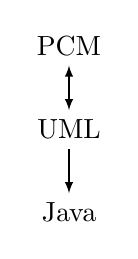
\begin{tikzpicture}
            \node[anchor=center] at (0,3em) (pcm) {PCM};
            \node[anchor=center] at (0,0em) (uml) {UML};
            \node[anchor=center] at (0,-3em) (java) {Java};
            \draw[latex-latex] (pcm) -- (uml);
            \draw[-latex] (uml) -- (java);
        \end{tikzpicture} & 
        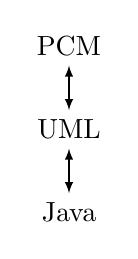
\begin{tikzpicture}
            \node[anchor=center] at (0,3em) (pcm) {PCM};
            \node[anchor=center] at (0,0em) (uml) {UML};
            \node[anchor=center] at (0,-3em) (java) {Java};
            \draw[latex-latex] (pcm) -- (uml);
            \draw[latex-latex] (uml) -- (java);
        \end{tikzpicture} & 
        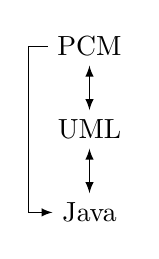
\begin{tikzpicture}
            \node[anchor=center] at (0,3em) (pcm) {PCM};
            \node[anchor=center] at (0,0em) (uml) {UML};
            \node[anchor=center] at (0,-3em) (java) {Java};
            \draw[latex-latex] (pcm) -- (uml);
            \draw[latex-latex] (uml) -- (java);
            \draw[-latex] (pcm.west) -- ++(-0.7em,0) |- (java);
            %\draw[-latex] (pcm.north) |- ++(-2em,0.7em) |- ([yshift=-0.7em]java.south) -- (java);
        \end{tikzpicture} & 
        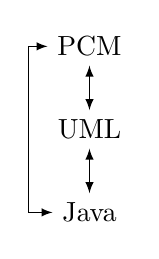
\begin{tikzpicture}
            \node[anchor=center] at (0,3em) (pcm) {PCM};
            \node[anchor=center] at (0,0em) (uml) {UML};
            \node[anchor=center] at (0,-3em) (java) {Java};
            \draw[latex-latex] (pcm) -- (uml);
            \draw[latex-latex] (uml) -- (java);
            \draw[latex-latex] (pcm.west) -- ++(-0.7em,0) |- (java);
        \end{tikzpicture} \\
        \midrule
        Transformation Incorrectness & 5 & 2 & 4 & 1 \\
        Missing Synchronization     & 0 & 0 & 6 & 7 \\
        Incompatible Constraints  & 0 & 0 & 2 & 2 \\
        Incompatible \newline Option Selection & 0 & 0 & 0 & 0 \\
        \bottomrule
    \end{tabular}
    \caption[Mistake types by case study phase]{Number of occurrences of different mistake types by the phase of the network case study with the stepwise addition of unidirectional transformations.}
    \label{tab:correctness_evaluation:errors:mistakes_by_phase}
\end{table}

The expected result is that synchronization mistakes first occurred when a cycle of the unidirectional transformations occurs which does not only consist of the cycle within one bidirectional transformations.
Only in that setting a synchronization scenario occurs which requires transformations to consider that other transformations may have created elements in both models.
Additionally, also errors at the network levels only occurred in those stages, although they could already occur in a linear network, like they also occurred in the single transformation case study, in which already the unidirectional consistency relations could be incompatible.



We had to perform two iterations of the previously described process.
In the first iteration, we faced failures due to mistakes at the operationalization level, whereas in the second iteration only failures due to remaining mistakes at the modularization level occurred.
We have tagged the states before and after the evaluation process in the GitHub repository~\cite{vitruvCBSEGithub}.

%\compactsubsection{Classification}

In the first iteration, all 187 tests failed.
The reason was that all transformations assumed that new elements are only created by the user or the transformation itself.
In consequence, we observed multiple instantiations and insertions in 187 cases, which we could trace back to 35 missing matchings of elements in the transformations.
After adding appropriate matchings, all these failures disappeared in a second iteration, so for the first iteration $\mathit{identifiedFailureRatio = resolvedFailureRatio = 1}$, since all detected failures were identified and resolved.

In the second iteration, 5 new failures occurred.
Three of them were diverging loops, which were caused by a namespace repeatedly prefixed to the name of classes, interfaces and enumerations in Java.
The causing mistakes were incompatible constraints: The Java model contains the fully qualified name of a class, whereas the UML model only contains the simple name, which was correctly propagated from UML to Java, but the namespace prefix was not removed in the opposite direction.
The two other failures were alternating loops, which were caused by alternations of element visibilities.
For methods and constructors, the visibilities were repeatedly changed due to an inconsistent mapping of visibilities from UML to Java and vice versa.
%After fixing the mistakes, two failures remained.
%Nevertheless, the reason for that were technical issues with the transformation engine due to its propagation of atomic changes.
%Since the original failures also disappeared in this case, we again have $identifiedFailureRatio = resolvedFailureRatio = 1$, since all detected failures were identified and resolved.
After fixing those mistakes, no failures remained.
So we again have $\mathit{identifiedFailureRatio = resolvedFailureRatio = 1}$, since all detected failures were identified and resolved. 

Summarizing, we were able to classify and resolve all failures in the case study and trace them back to mistakes with our classification in \autoref{chap:errors}.
This demonstrates the applicability of our categorization and is an indicator for the completeness and correctness of our catalog.
Most important, we did not find any failures that were caused by mistakes at a different specification level than we expected.
To further validate the catalog, we should apply it to further case studies.
It is however hard to find existing, independently developed transformations between at least three metamodels.
They would have to be developed in a schema similar to the one proposed by \textcite{kramer2016c}.
%\todoHeiko{Irgendwie noch sagen, dass wegen das wegen dem hohen Aufwand kein Threat to Validity ist? Oder kommt das nicht gut an?}
%\todoHeiko{Generell mehr Threats to Validity diskutieren?}


\todo{Erkennntis aus Iterationen: Solange wir nur einen Baum von Relationen haben, gibt es keine Fehler auf Modularisierungsebene (keine Inkompatibilitäten), diese kommen erst bei Zyklus hinzu (allerdings schon bei internem Zyklus durch Unidirektionalität?). D.h. wie schon voher angegeben sind Inkompatibilitäten per Konstruktion vermieden, wenn wir nur einen Baum von Relationen haben.
Falls wir keinen Baum garantieren können: In this case, the consistency specifications must be revised whenever non-termination or non-deterministic termination of consistency preservation is observed (see \autoref{fig:correctness:categorization})}



%\compactsubsection{Element Matching}

%In \autoref{sec:avoiding:matching}, we presented three levels of matching equal elements across different transformation paths.
%We used our case study to investigate, which of those levels are necessary in a practical scenario.

\end{copiedFrom} % ICMT


\subsection{Discussion}

Erkenntnis: Immer erst Fehler auf Transformationsebene fixen, da diese Fehler auf den anderen Ebenen verdecken.

Erkenntnis: Was wir nicht ausschließen können sind Fehler in den Konsistenzrelationen, die auf der unterschiedlichen Interpretation von Konsistenz basieren. Wenn beispielsweise die Relation UML<>PCM das Repo klein schreibt, Java<>PCM aber das Repo groß schreibt, wird das (korrekterweise) nicht gemacht.
Hier ist eine andere Auffassung von Korrektheit verletzt (Korrektheit der modularen bzgl. einer einheitlichen globalen Spezifikation), da implizit vorausgesetzt wird, dass in einem globale Verständnis in beiden Fällen auf das gleiche Repository abgebildet wird. (siehe Figure 6.4 in MA Timur).
Dies war explizit nicht die Art von Korrektheit die wir betrachtet haben, da sie ein anderes Ziel verfolgt. Sie erfordert Kenntnis über die übergeordnete Semantik der Elemente, beispielsweise durch eine globale Konsistenzspezifikation, gegen die man das prüft (siehe entsprechendes Kapitel) oder durch die Abbildung auf einen gemeinsamen Formalismus, der verifizierbar ist.

In Timurs MA außerdem betrachtet wie sich eine Kategorisierung in too many, incorrect and too few elements auf failures auswirkt. Hieraus konnten jedoch keine relevanten Erkenntnisse gezogen werden, weshalb wir es hier nicht diskutieren und auf die MA verweisen (Table 5.2)


\subsubsection{Threats to Validity}
- The transformation were not constructed synchronizing, thus obviously many synchronization errors occur. If the scenario is foreseen, there may be much less errors at this level and more at the others -> need to perform further evaluation were developer know about necessity to use transformations in a network to properly construct them and then see how often that still fails. (future work)


\paragraph{User Interaction}
Erlaubt Java->PCM, dass man an beliebiger Stelle ein Interface anlegen kann. PCM-UML erlaubt das nur im contracts-Package. Erstellt man ein Interface in einem anderen Package, erstellt PCM-UML nochmal eines im contracts Package, dadurch auch UML-Java und dann matcht UML-PCM, wodurch es bei PCM-Java zwei Abbildungen des Interface gibt. Hier haben wir inkompatible Constraints, aber wenn die Nutzerabfrage für das Matching in beiden Transformationen PCM-Java und PCM-UML eingebaut wird, kann der Nutzer konfligierende Entscheidungen treffen. Um das zu verhindern, müssten die Transformationen aufeinander abgestimmt werden.

Generell: Nutzerinteraktion lässt sich bei den Relationen dadurch ausdrücken, dass alle Auswahloptionen als valide consistency relation pairs betrachtet werden.
Problematisch sind jedoch die consistency preservation rules, da sie es potentiell erlauben konfligierende der condition elements auszuwählen, genauso wie es bei den Transformationen selbst auch passieren kann.
Wir haben diese selection of options im Orchestrierungs-Kapitel diskutiert.
Hier ist definitiv noch Future Work notwendig um zu untersuchen, wie man Nutzerentscheidungen über mehrere Transformationen hinweg miteinander alignen kann \todo{Future Work}.
Generell ist eine Untersuchung des Alignments von CPRs sinnvolles \todo{Future Work}.


Limitierung: Hier wenig Optionsauswahl, d.h. in den meisten Fällen entscheiden sich die Transformationen für ein Element und habe keine Auswahl.

Alignment der Transformationen: kein Threat, wurde per Konstruktion ausgeschlossen


\subsubsection{Limitations}
